%--------------------------------------
% Create title frame
\titleframe

%--------------------------------------
% Table of contents
\begin{frame}{Overview}
  \setbeamertemplate{section in toc}[sections numbered]
  \tableofcontents
\end{frame}

%--------------------------------------

\section{Power electronics interfaces}

\begin{frame}{3 main categories of power electronics devices}
    \begin{columns}
        \begin{column}{0.6\textwidth}
          \begin{itemize}
            \item \textbf{Rectifiers}: AC to DC, are typically used at the output of small wind turbines or micro-turbines
            \item \textbf{DC-DC converters} e.g. to interface photovoltaic modules and achieve their maximum power operating point
            \item \textbf{Inverters}: DC to AC e.g. to connect PV modules to the AC distribution grid
          \end{itemize}
        \end{column}
        \begin{column}{0.3\textwidth}
              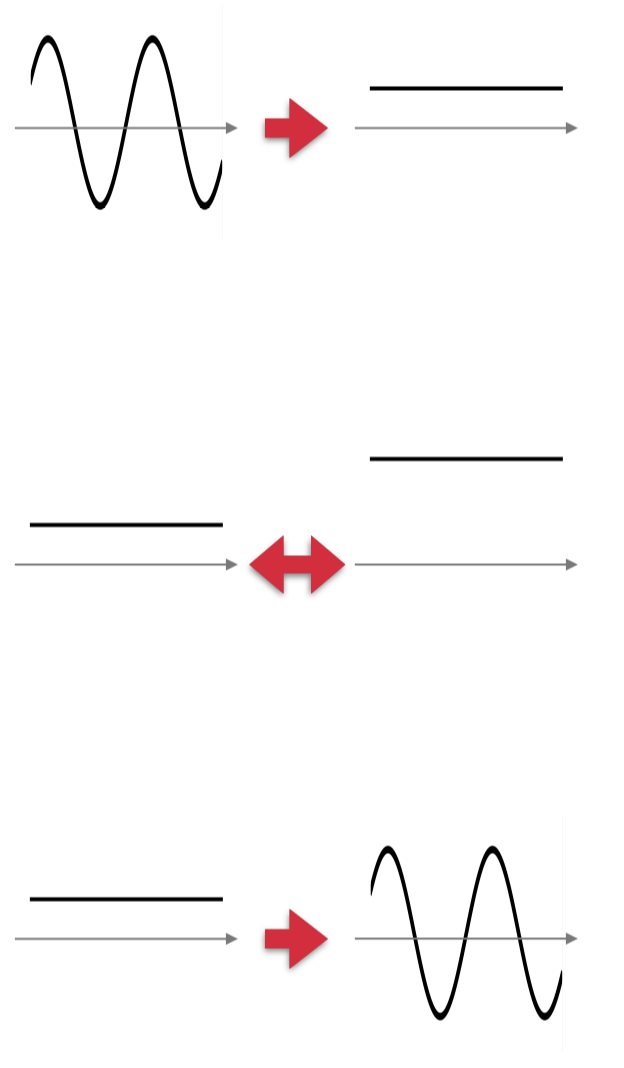
\includegraphics[width=\textwidth]{images/types_of_converters.png}
        \end{column}
    \end{columns}
\end{frame}

\begin{frame}{}
  \begin{block}{The main components of power electronics devices}
  Controllable switches that can be actuated at a high frequency, without excessive losses, and with a large lifetime  
  \end{block}
  \vspace{1cm}

  \begin{columns}
      \begin{column}{0.4\textwidth}
        Ideal switch model:
        \begin{itemize}
          \item no losses
          \item switches without delay
        \end{itemize}
      \end{column}
      \begin{column}{0.4\textwidth}
          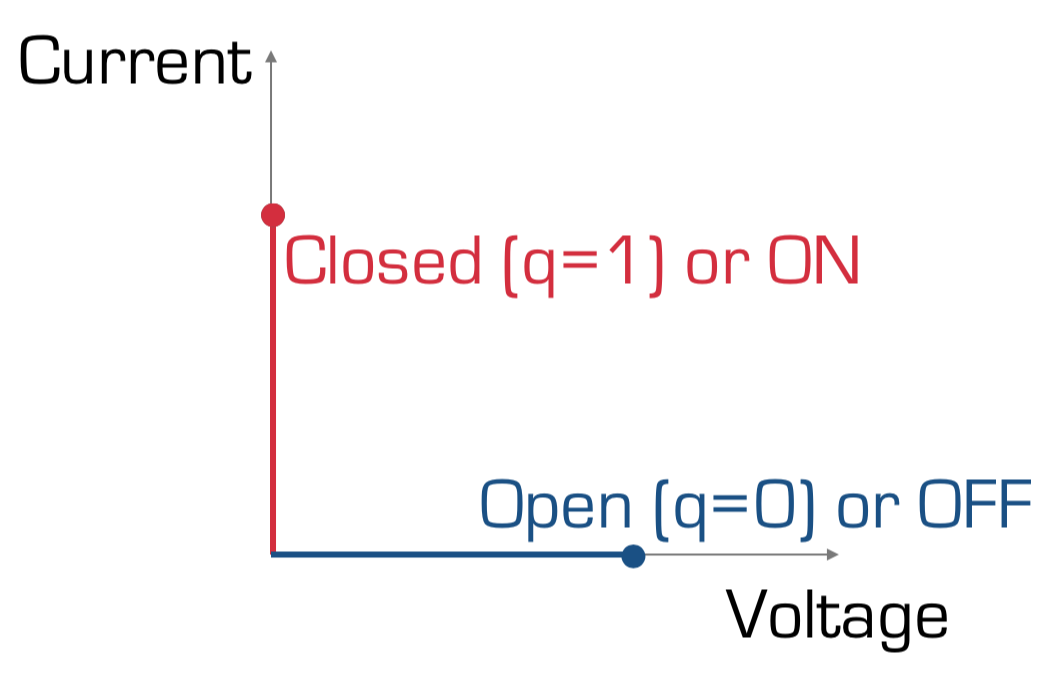
\includegraphics[width=\textwidth]{images/ideal_switch.png}
      \end{column}
  \end{columns}
\end{frame}

\begin{frame}{Realistic switch model}
  \centering
  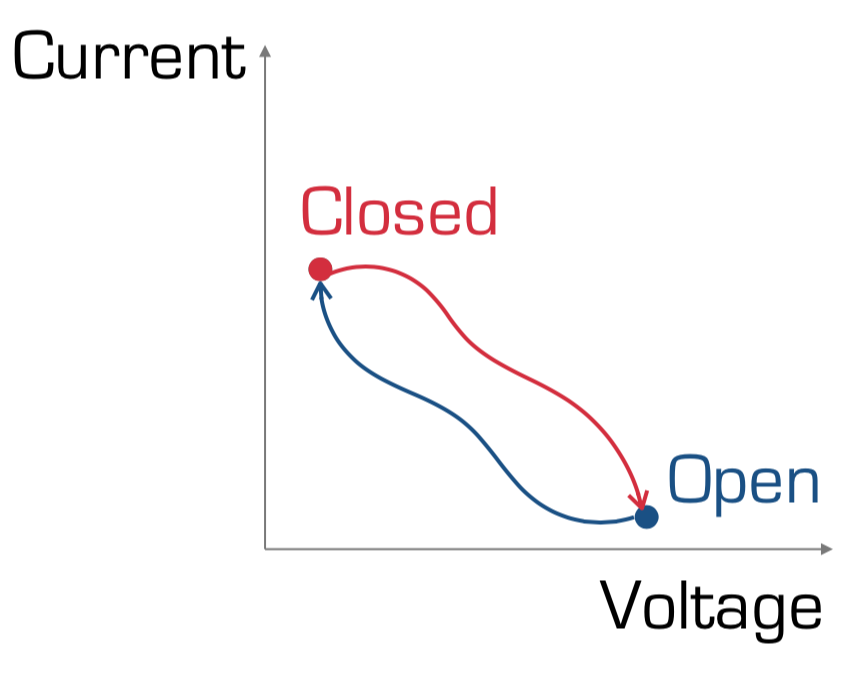
\includegraphics[width=0.4\textwidth]{images/realistic_switch.png}
\end{frame}

\begin{frame}{Diode models: ideal diode}
  \begin{center}
    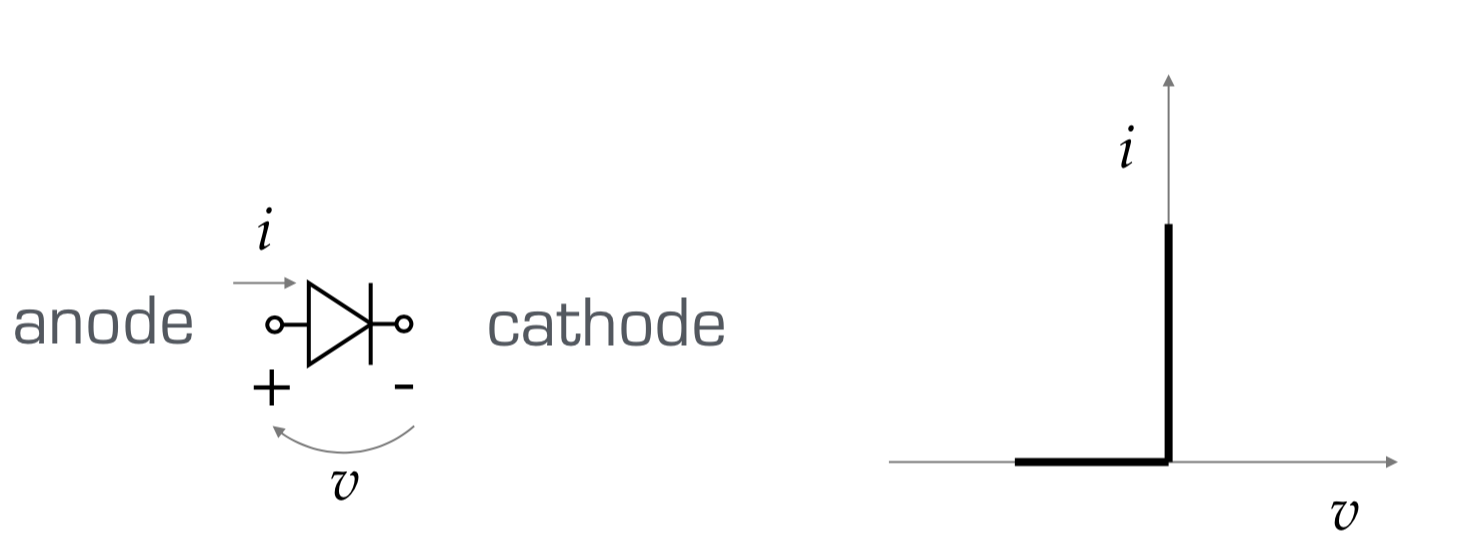
\includegraphics[width=0.6\textwidth]{images/ideal_diode.png}
  \end{center}
  \begin{itemize}
    \item Current flows from anode to cathode when forward biased: $i>0 \Rightarrow v=0$
    \item No current when reversed bias:  $v<0 \Rightarrow i=0$
  \end{itemize}
  Not really controllable, hence not suited for all applications.
\end{frame}

\begin{frame}{Diode models: realistic diode in the forward bias region}
  \begin{center}
    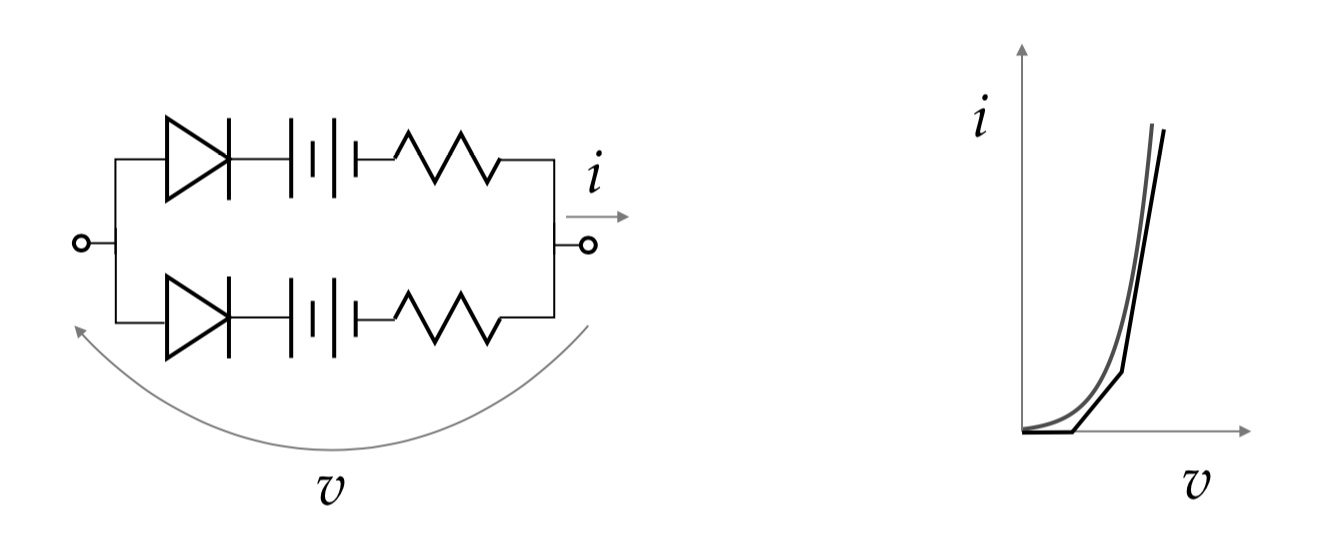
\includegraphics[width=0.6\textwidth]{images/piecewise_diode.png}
  \end{center}
Piecewise linear approximation of “true exponential model”.
\end{frame}

\begin{frame}{Thyristors}
  \begin{columns}
    \begin{column}{0.2\textwidth}
      \begin{center}
        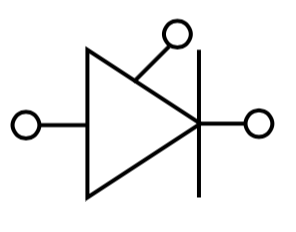
\includegraphics[width=\textwidth]{images/thyristor.png}
      \end{center}
      
    \end{column}
    \begin{column}{0.7\textwidth}
      \textbf{Thyristors are “controllable diodes”, through a gate where a signal is applied}\\[\baselineskip]

      Different types:
      \begin{itemize}
      \item GTO (gate turn off) can be turned on and off, less than 1kHz switching frequency
      \item SCR (silicon-controlled rectifier): can be turned on, turns off when forward current goes through zero
      \item TRIAC (Triode alternating current): two SCR back to back with one gate (AC-AC conversion)
      \end{itemize}
    \end{column}
  \end{columns}
\end{frame}

\begin{frame}{Transistors}
  \begin{columns}
        \begin{column}{0.45\textwidth}
  Bipolar junction transistors (BJT)
  \begin{center}
    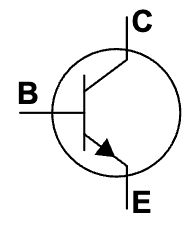
\includegraphics[width=0.25\textwidth]{images/BJT_symbol_NPN.png}
  \end{center}
  \begin{itemize}
    \item  Historically used as amplifiers in their active region of operation
    \item  Can also be used as a switch, in the saturation region
    \item  High power, but high losses
  \end{itemize}
  \end{column}

  \begin{column}{0.45\textwidth}
  Field effect transistors (MOSFET)  
  \begin{center}
    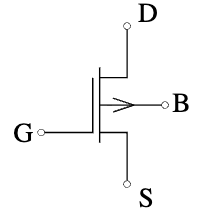
\includegraphics[width=0.25\textwidth]{images/Mosfet-zp.png}
  \end{center}
  \begin{itemize}
    \item  Historically used as amplifiers in their active region of operation
    \item  Can also be used as a switch, in the saturation region
    \item  High power, but high losses
  \end{itemize}
  \end{column}
  \end{columns}
\end{frame}

  \begin{frame}{Insulated Gate Bipolar Transistor (IGBT)}
    \begin{columns}
      \begin{column}{0.2\textwidth}
        \begin{center}
          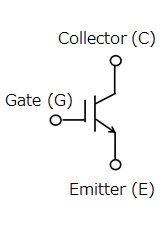
\includegraphics[width=\textwidth]{images/igbt-001_1_en.png}
        \end{center}
      \end{column}
      \begin{column}{0.7\textwidth}
        \begin{itemize}
          \item Most common device for high power DC-DC converters and inverters from medium to high voltages
          \item Combination of BJT and MOSFET
          \item Now replaces thyristors in most medium to high power applications
        \end{itemize}
      \end{column}
    \end{columns}
  \end{frame}
  

\begin{frame}{Characterization of power electronics devices}
    \begin{columns}
        \begin{column}{0.5\textwidth}
          \textbf{DC component}:
          \begin{itemize}
            \item Integral of the output signal over a full AC input cycle.
            \item In case of a rectifier, this is the power that is really transmitted from source to load.
          \end{itemize}
        \end{column}
        \begin{column}{0.5\textwidth}
          \textbf{Total Harmonic Distortion}: THD = ratio of the total signal, including harmonics, to the desired frequency component:
          $$THD = \sqrt{\frac{F_{R M S}^2-F_{R M S, 1}^2}{F_{R M S}^2}}$$

          \textit{\small For low-voltage systems (\(\le 1\) kV), the generally accepted maximum THD limit for voltage is 8\% according to IEEE 519-2022 and EN 50160 standards, though 5\% is often the recommended design target for better power quality. }
        \end{column}
    \end{columns}
\end{frame}

\begin{frame}{Rectifiers}
  \begin{center}
    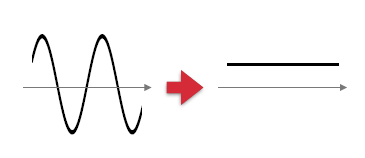
\includegraphics[width=0.2\textwidth]{images/rectifiers.png}
  \end{center}

  Rectifiers: large subclass of topologies for AC to DC conversion
  \begin{itemize}
    \item Single-phase or three phase voltage source to DC current load
    \item Power-electronic is “only” the front end:
  \end{itemize}

  \begin{center}
    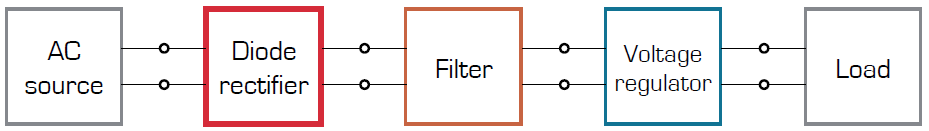
\includegraphics[width=0.7\textwidth]{images/cascade.png}
  \end{center}

\end{frame}


\begin{frame}{Half bridge single phase topology}
  \begin{center}
    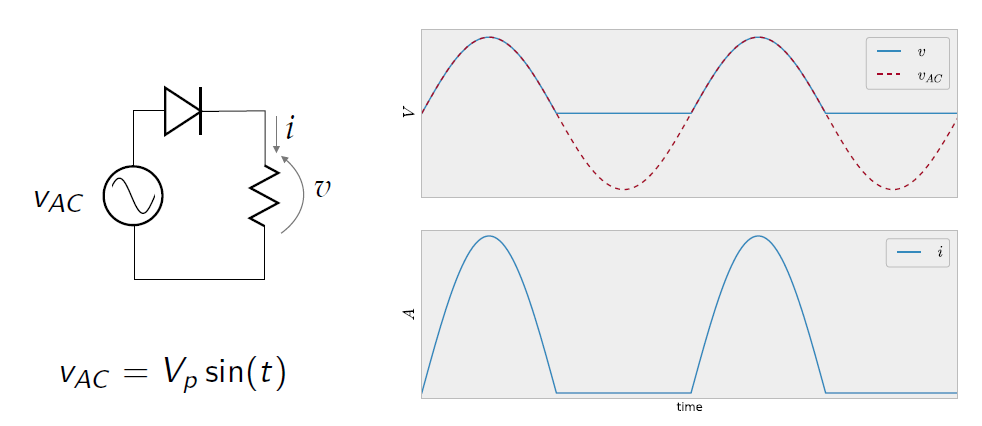
\includegraphics[width=0.7\textwidth]{images/half_bridge_1P.png}
  \end{center}

    DC component: $$V_{D C}=\frac{V_p}{2 \pi} \int_0^\pi \sin (t) d t=-\left.\frac{V_p}{2 \pi} \cos (t)\right|_0 ^\pi=\frac{V_p}{\pi}$$
\end{frame}

\begin{frame}{Full-bridge single phase topology}
  \begin{center}
    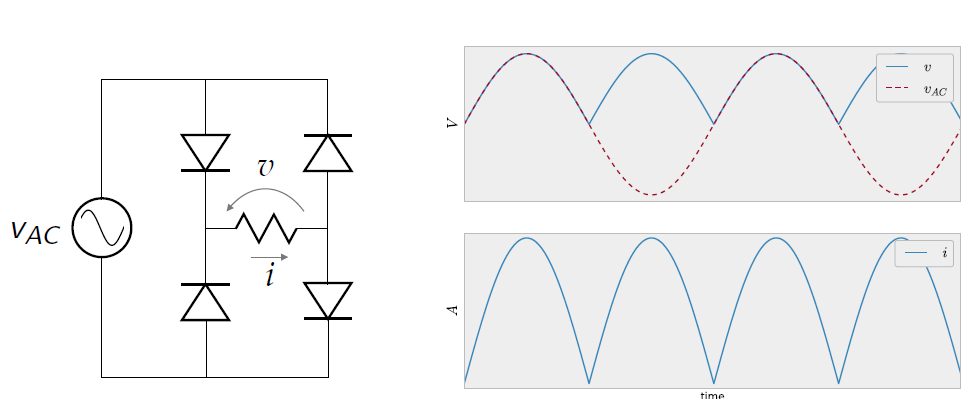
\includegraphics[width=0.7\textwidth]{images/full_bridge_1P.png}
  \end{center}

  \begin{itemize}
    \item DC component twice of the half bridge
    \item But large harmonic current in the input AC current
    \item DC output not controllable
  \end{itemize}
\end{frame}

\begin{frame}{Full-bridge single phase topology with low pass filter}
  \begin{center}
    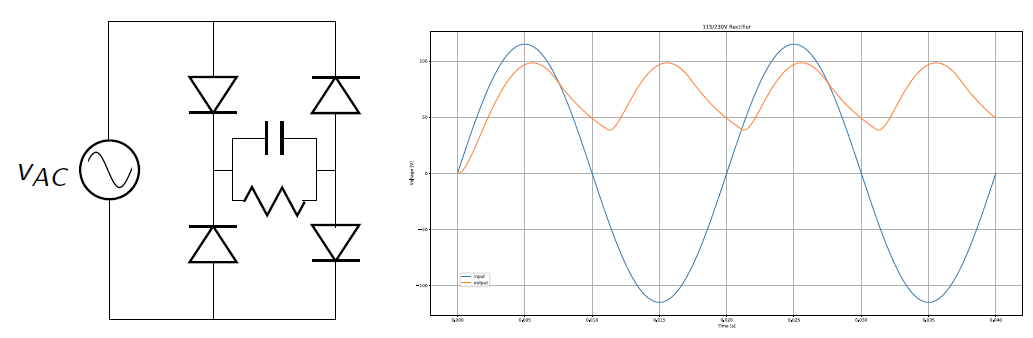
\includegraphics[width=0.7\textwidth]{images/full_bridge_1P_filter.png}
  \end{center}
  \begin{itemize}
    \item  Improves output harmonics content
    \item  Better if capacitor size increases, which in turn degrades harmonic content of input
    \item  Bad power factor $\Rightarrow$ LC topology
    \item  Active power factor correction $\Rightarrow$ DC-DC after the rectifier
  \end{itemize}
\end{frame}

\begin{frame}{Recap with more realistic components}
  \centering
  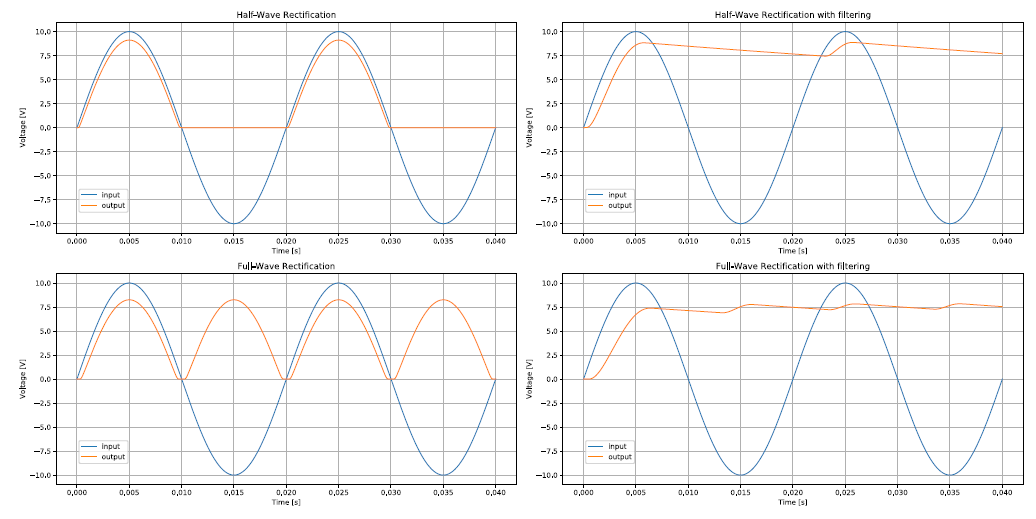
\includegraphics[width=0.9\textwidth]{images/recap_rectifiers.png}
\end{frame}


\begin{frame}{6-pulse rectifier (3-phase source)} 
  \centering
  \href{https://youtu.be/WVI8Z7p_rdY}{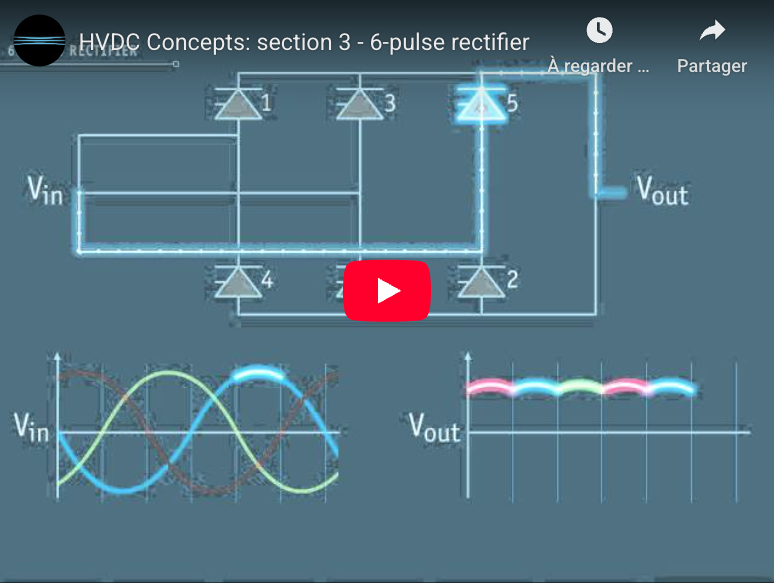
\includegraphics[width=0.6\textwidth]{images/video_6pulse_rectifier.png}}
\end{frame}


\begin{frame}{DC - DC converters}
  \begin{center}
    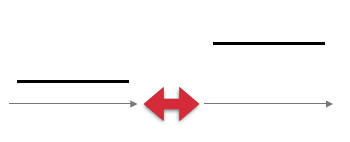
\includegraphics[width=0.4\textwidth]{images/DCDC.png}
  \end{center}
  \begin{itemize}
    \item DC-DC converters are present in many devices, from mW power level to MW level
    \item Made possible by MOSFET and IGBTs
    \item Can be unidirectional, from low voltage to high voltage or the inverse, or bidirectional: 
    $$v_h > v_l, \ i_l > i_h$$
  \end{itemize}
\end{frame}

\begin{frame}{Basic bloc: two switches}
  \begin{center}
    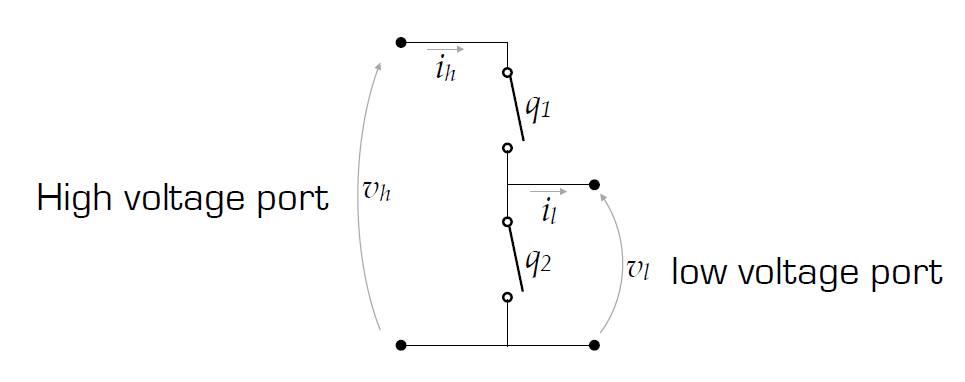
\includegraphics[width=0.8\textwidth]{images/principle_DCDC.png}
  \end{center}
  \begin{itemize}
    \item Only one switch \alert{ON} at a time!
    \item Pulse Width Modulation (PWM) is the process that actuates the switches (duty cycle signal compared to a reference triangular waveform of a chosen frequency)
  \end{itemize}
\end{frame}

\begin{frame}{Converter types}
    \begin{columns}
        \begin{column}{0.5\textwidth}
          BUCK\\
          $q_1$ is a controllable switch and $q_2$ is a diode
          \begin{center}
            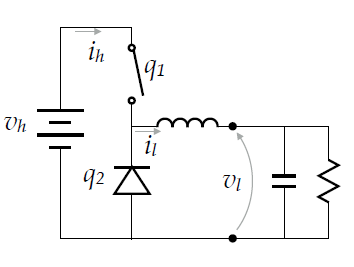
\includegraphics[width=0.5\textwidth]{images/buck1.png}\\
            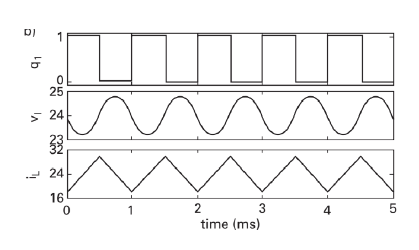
\includegraphics[width=0.5\textwidth]{images/buck2.png}
          \end{center}
          $v_h=48V$, duty cycle$=50 \%$
        \end{column}
        \begin{column}{0.5\textwidth}
          BOOST\\
          $q_1$ is a diode and $q_2$ is a controllable switch
          \begin{center}
            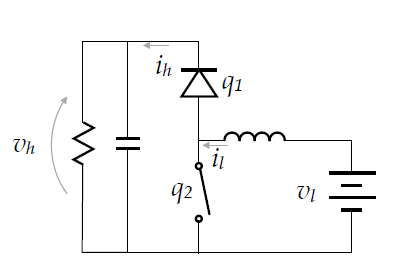
\includegraphics[width=0.5\textwidth]{images/boost1.png}\\
            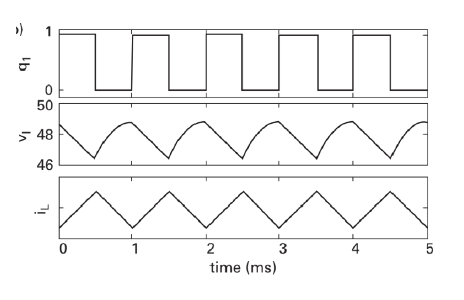
\includegraphics[width=0.5\textwidth]{images/boost2.png}
          \end{center}
          $v_l=24V$, duty cycle$=50 \%$
        \end{column}
    \end{columns}
\end{frame}



\begin{frame}{Inverters}
  \begin{center}
    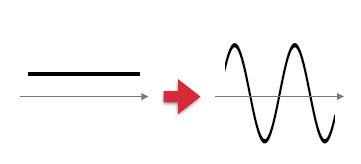
\includegraphics[width=0.3\textwidth]{images/inverters.png}
  \end{center}
  \begin{itemize}
    \item 
  \end{itemize}
    \begin{center}
    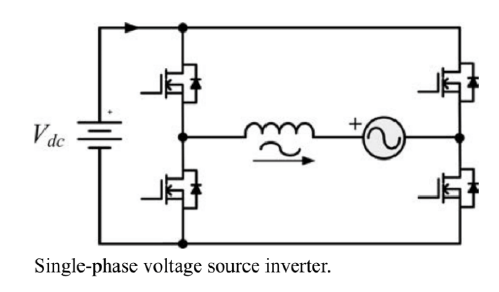
\includegraphics[width=0.5\textwidth]{images/principle_inverter.png}
  \end{center}

\end{frame}




\begin{frame}{How an inverter works}
  \centering
  \href{https://youtu.be/qVeERT4nyz8}{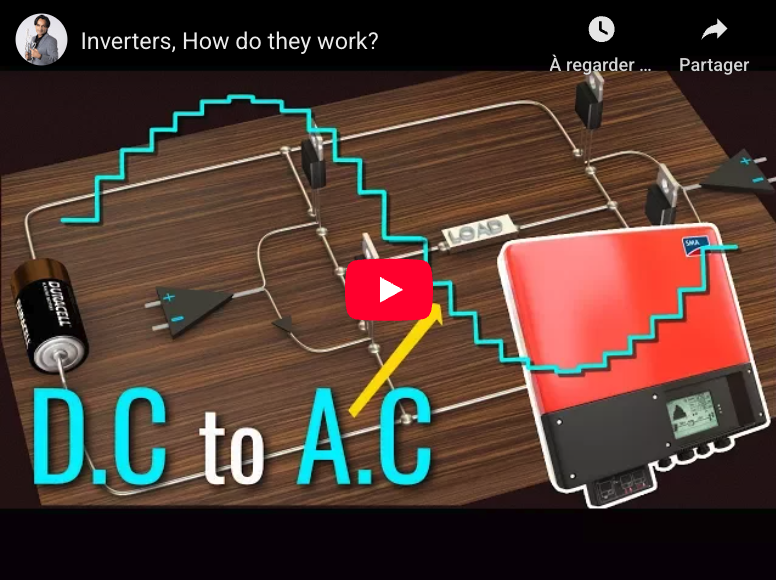
\includegraphics[width=0.6\textwidth]{images/video_inverter.png}}
\end{frame}


\begin{frame}{6-pulse inverter (3-phase)}
  \centering
  \href{https://youtu.be/jOquS6uqpeY}{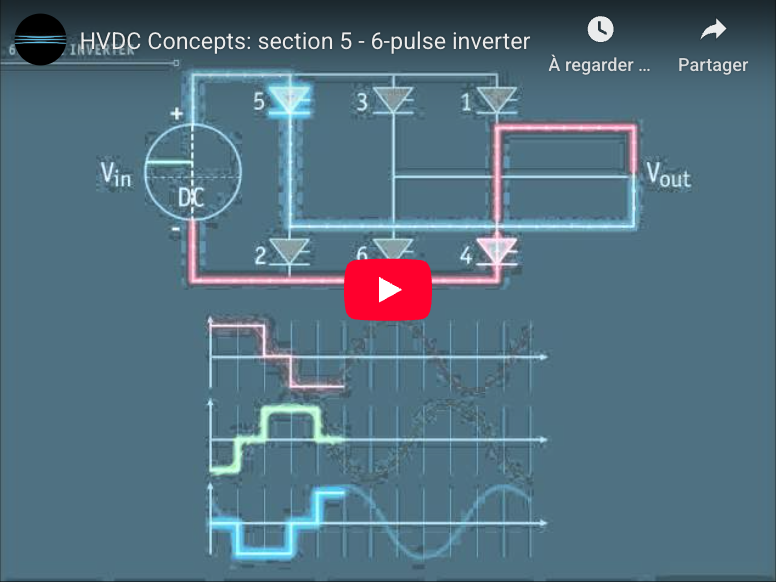
\includegraphics[width=0.6\textwidth]{images/video_6pulse_inverter.png}}
\end{frame}

\section{Power generation sources}

\subsection{Wind turbines}

\begin{frame}{Wind turbines}
\begin{itemize}
  \item Wind turbines convert the mechanical power of wind into electrical power.
  \item The power of the wind can be derived from its kinetic energy
$$
E_{w}=\frac{1}{2} m v^{2}
$$
As power is the time derivative of energy, we have, assumming the speed is constant:
$$
P_{w}=\frac{d E_{w}}{d t}=\frac{1}{2} \frac{d m}{d t} v^{2}
$$
And $\frac{d m}{d t}=\rho A v$ with $A$ the area crossed by the wind, and $\rho$ is the mass of air by unit of volume. This yields
$\boxed{P_{w}=\frac{1}{2} \rho A v^{3}}$.
\end{itemize}
\end{frame}

\begin{frame}{Power conversion}
Only a fraction of the wind power is harvested by the blades. Actually, the energy harvested is function of the \textbf{speed of the air that enters the blades}, $v_{u}$, and \textbf{speed of the air that leaves the blades}, $v_{d}$ :
$P_{b}=\frac{1}{2} \frac{d m}{d t}\left(v_{u}^{2}-v_{d}^{2}\right)$

Approximating $\frac{d m}{d t}$ by $\rho A \frac{v_{u}-v_{d}}{2}$ and defining the coeffitient $\lambda_{w}$ as
$
\lambda_{w}=\frac{v_{d}}{v_{u}}
$, 
then the power \textbf{harvested} by the turbine can be written as
$$
\boxed{P_{b}=\frac{1}{2} \rho A \frac{v_{u}-\lambda_{w} v_{u}}{2}\left(v_{u}^{2}-\lambda_{w}^{2} v_{u}^{2}\right)}
$$

\end{frame}

\begin{frame}{Turbine efficiency}
If we define the coefficient
$
C_{p}=\frac{1}{2}\left(1+\lambda_{w}\right)\left(1-\lambda_{w}^{2}\right)
$, then
$$
\boxed{P_{b}=\frac{1}{2} C_{p} \rho A v_{u}^{3}}
$$

\textbf{Betz limit:}
\begin{itemize}
  \item It can be shown that there is a theoretical limit for $C_{p}$ at
\end{itemize}
$$
\frac{16}{27}=59.2 \%
$$
\begin{itemize}
  \item This limit is reached for $\lambda_{w}=1 / 3$.
\end{itemize}

\end{frame}

\begin{frame}{Efficiency of different technologies as a function of tip-speed ratio (TSR)}
\begin{center}
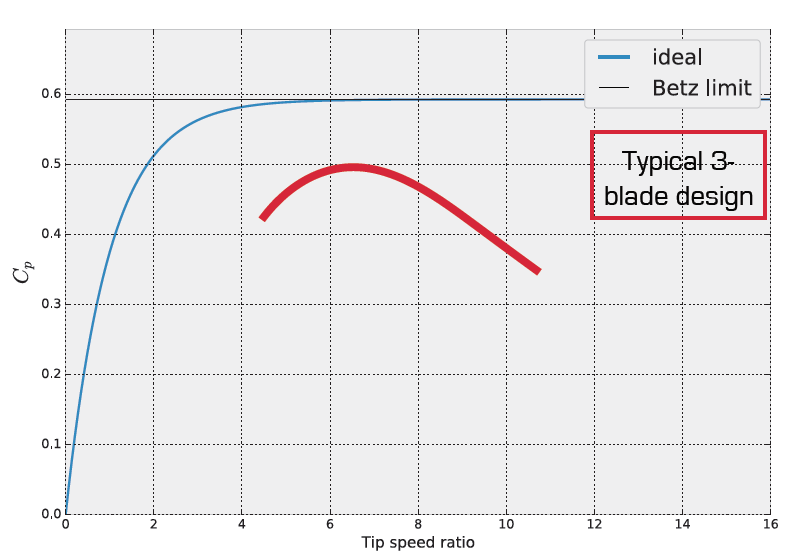
\includegraphics[width=0.5\textwidth]{images/Betz.png}\\
TSR = rotor tip speed / wind speed.
\end{center}

\end{frame}

\begin{frame}{Electromechanical conversion}
\begin{center}
  \href{https://youtu.be/JJr4PIuQp2w}{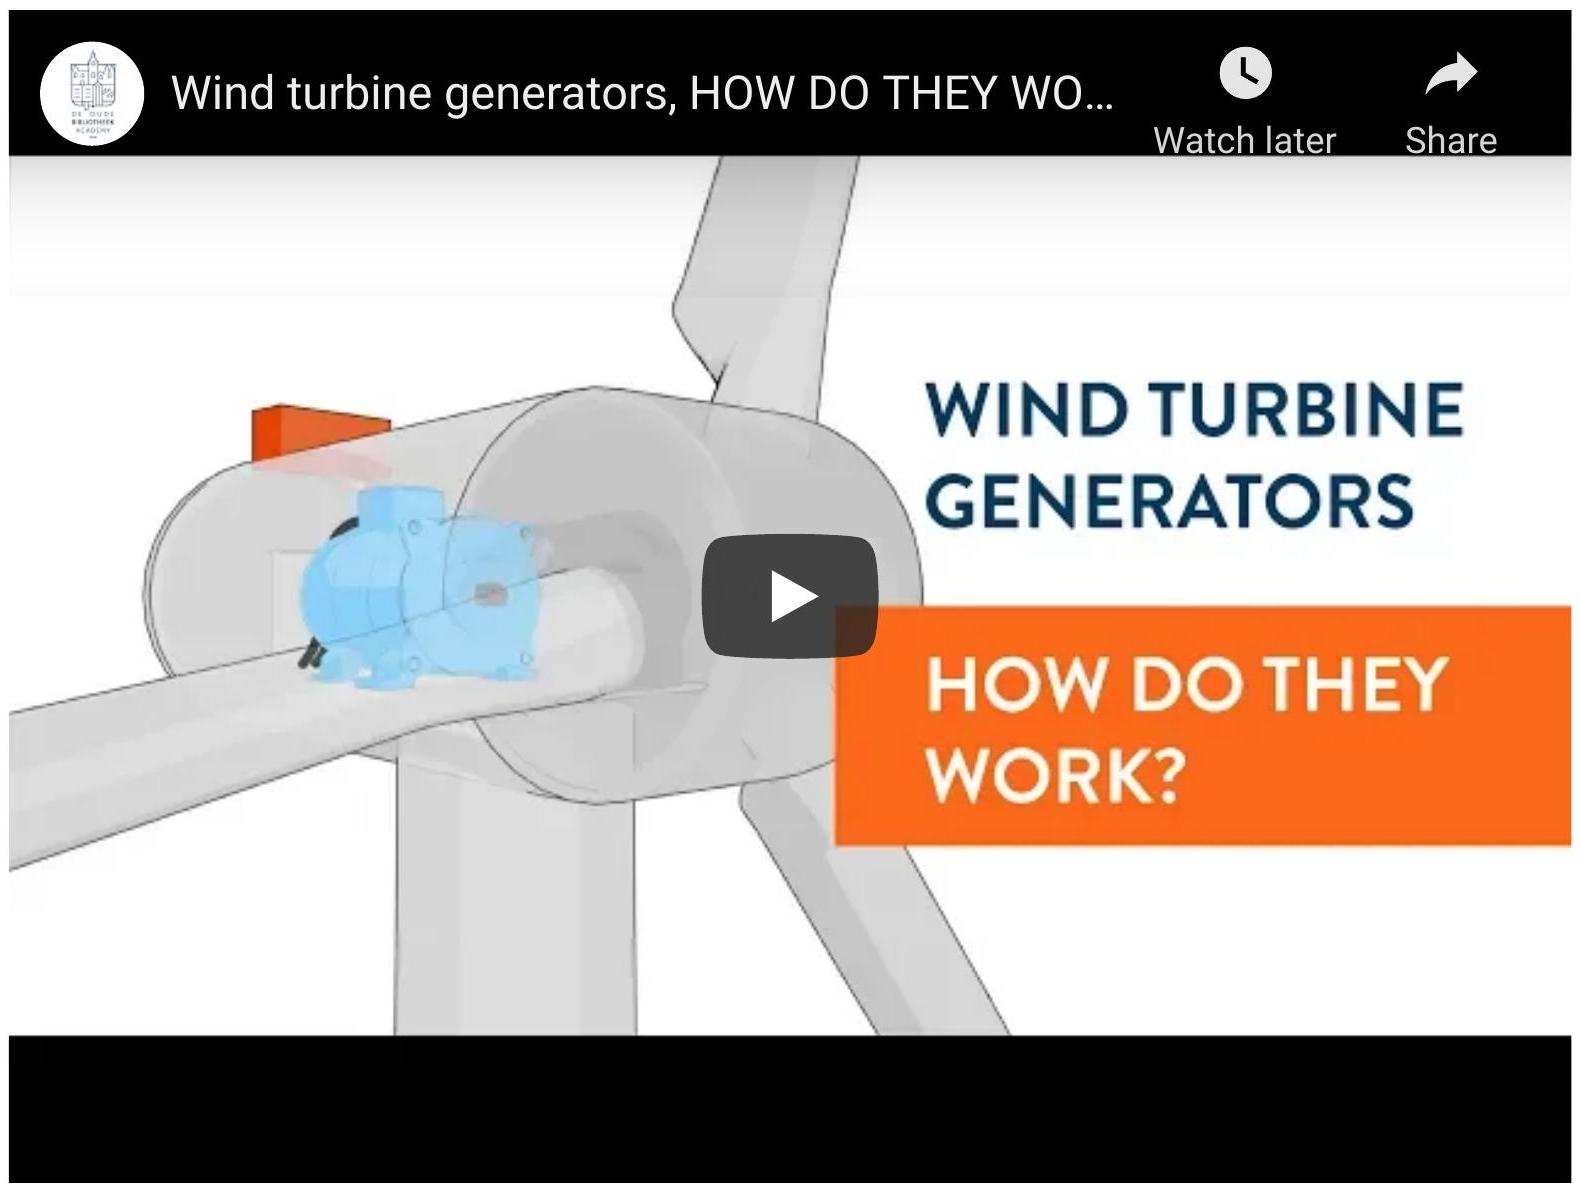
\includegraphics[width=0.5\textwidth]{images/video_wind.jpg}}
\end{center}

\end{frame}

\begin{frame}{Electromechanical conversion}
So far, we have only been talking about mechanical power conversion!\\
Several types of generators can be used to convert mechanical power into electrical power:
\begin{itemize}
  \item Synchronous machine
  \item DC machine
  \item Induction machine
  \item Doubly fed induction machine
\end{itemize}

Brushless variants of (some of) these machines can be used to decrease maintenance needs, through permanent magnets. 
Those cannot be used for large size generators (> several hundreds of kW).
\end{frame}

\begin{frame}{Power electronics interface}
Most of the time, and especially in microgrids operation, these generators are coupled with power electronics to generate power with an appropriate shape:
\begin{itemize}
  \item the output of the generator goes through a DC convertion stage (rectifier if AC generator, DC-DC if DC generator) to cope with wind speed variations
  \item if the distribution grid is AC , then there is an additional inverter stage.
\end{itemize}
\end{frame}

\begin{frame}{Power electronics are also used}
  \begin{columns}
    \begin{column}{0.5\textwidth}
      \begin{itemize}
        \item to maximize the energy harvested, especially for low-to-medium power generators (instead of adapting rotor speed through e.g. controlling blade pitch):
        \item to limit the power output at high wind speeds to avoid degradation
      \end{itemize}
    \end{column}      

    \begin{column}{0.5\textwidth}
      \begin{center}        
        Wind generator operating characteristic \\
        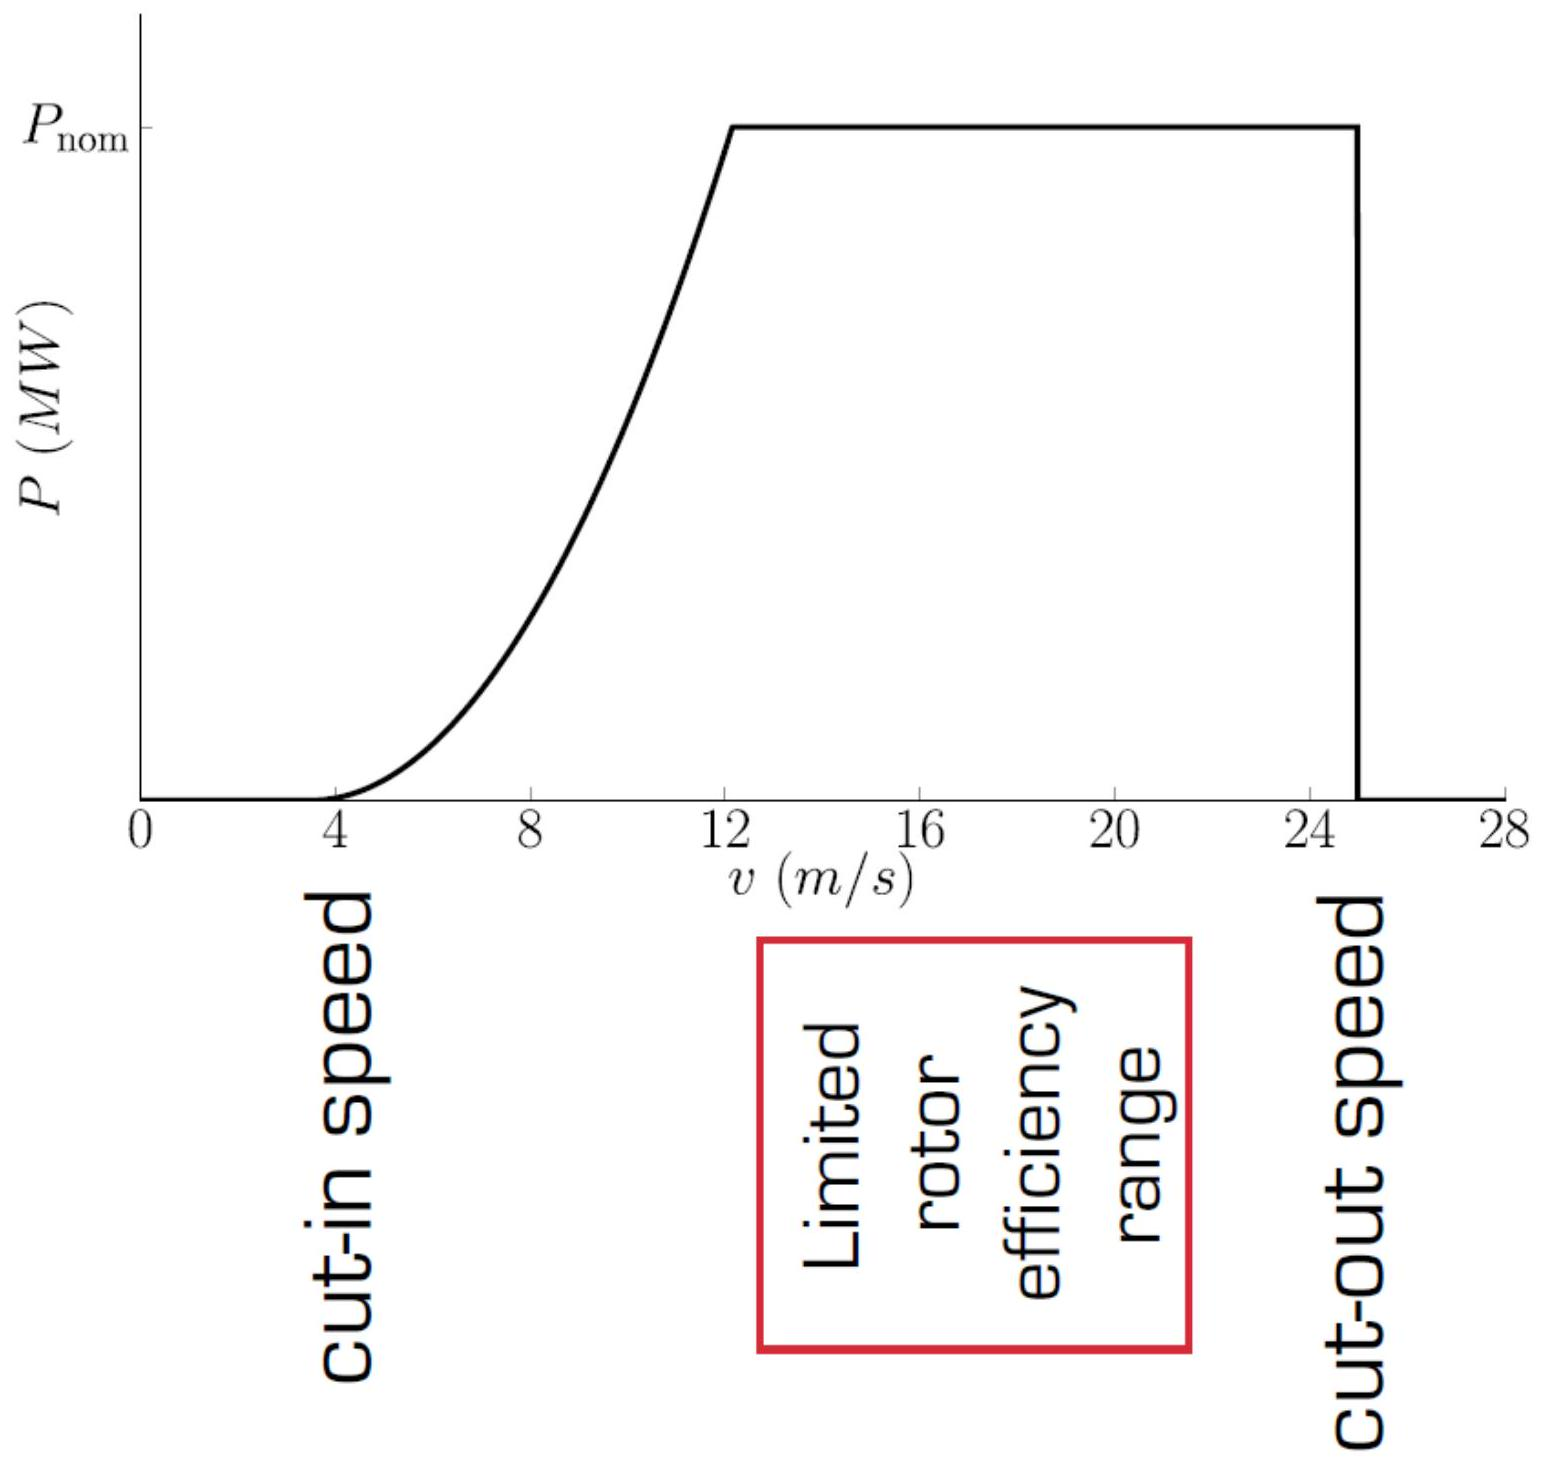
\includegraphics[width=0.9\textwidth]{images/P_vs_wind.jpg}
      \end{center}
    \end{column}
  \end{columns}
\end{frame}


\subsection{Photovoltaic generation}
\begin{frame}{Photovoltaic generation}
A PV cell is composed of semiconductor material. Photons emitted by the sun interact with the semiconducting material in two ways:

\begin{columns}
    \begin{column}{0.5\textwidth}
    \begin{enumerate}
      \item photons directly transmit energy to electrons and allow them to move into the conduction band.
      \item a thermally generated current as in a p -n junction (diode).\\
    \end{enumerate}
    \end{column}      
    \begin{column}{0.5\textwidth}
      \begin{center}        
      \href{https://youtu.be/L_q6LRgKpTw}{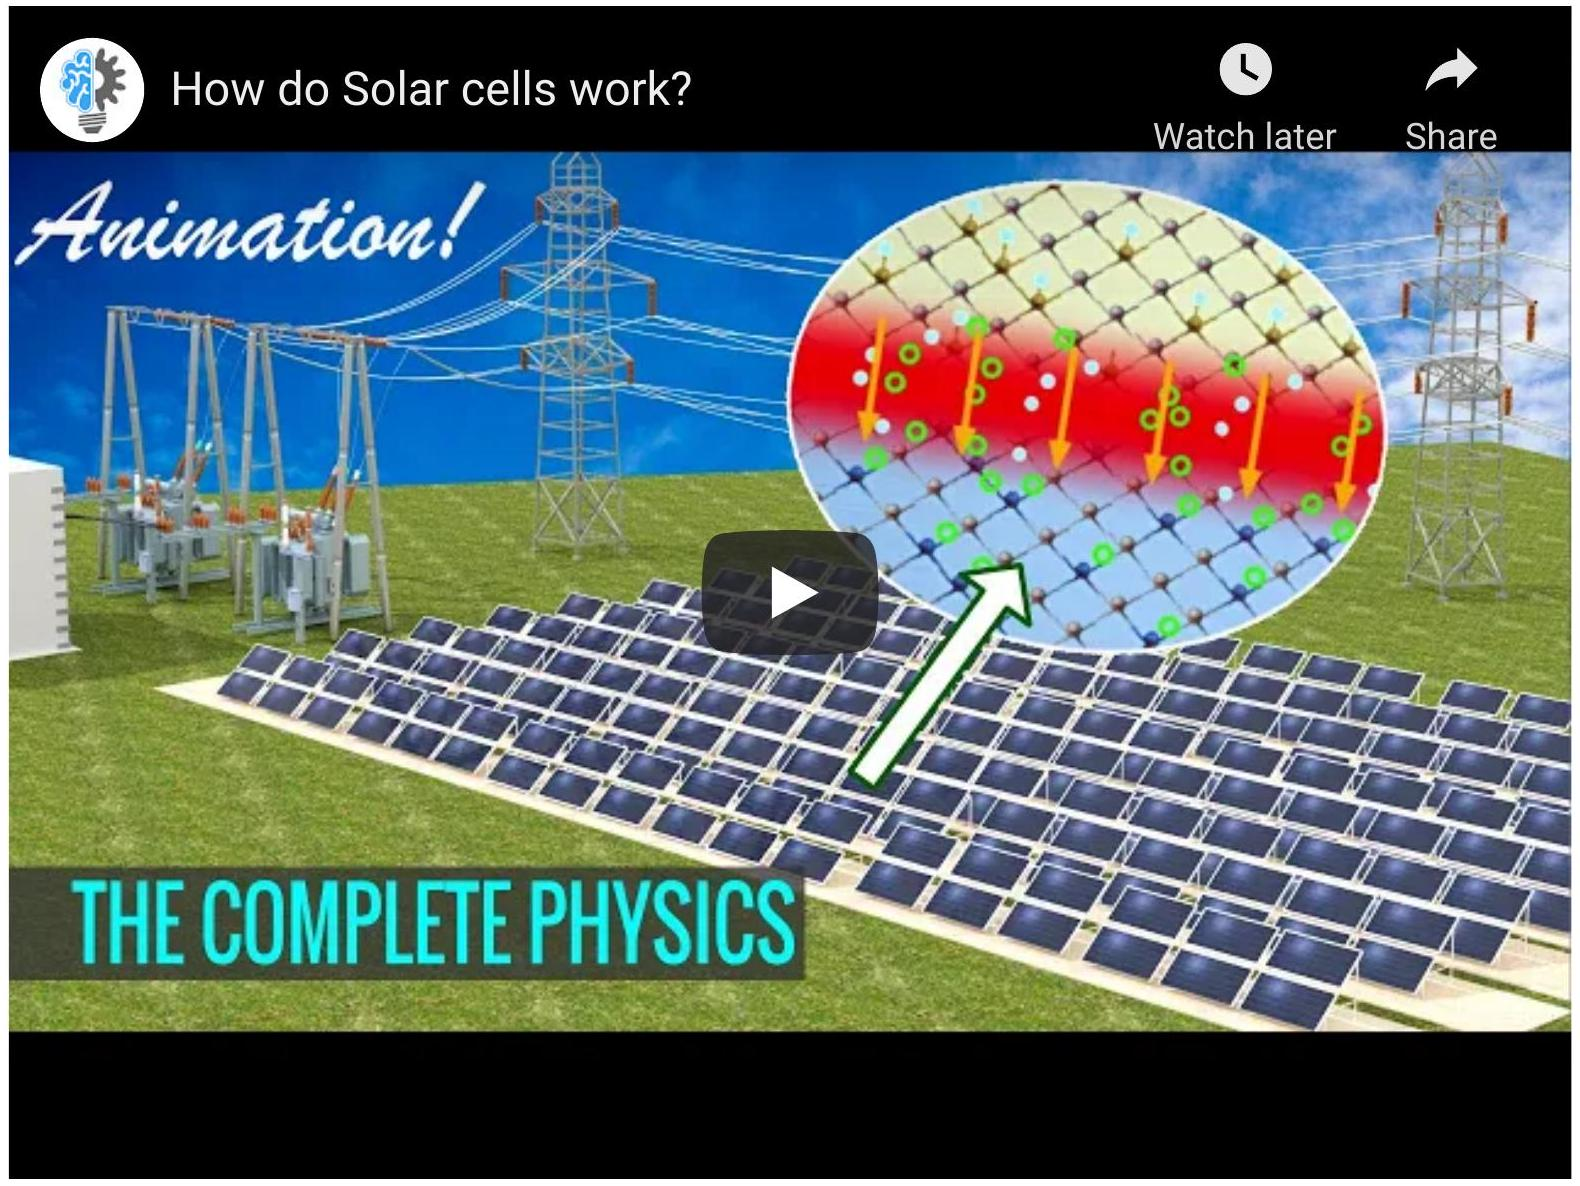
\includegraphics[width=0.8\textwidth]{images/video_PV.jpg}}
      \end{center}
    \end{column}
  \end{columns}
\end{frame}

\begin{frame}{Effect of temperature and irradiance}
\begin{columns}
  \begin{column}{0.5\textwidth}
    Effect of temperature
    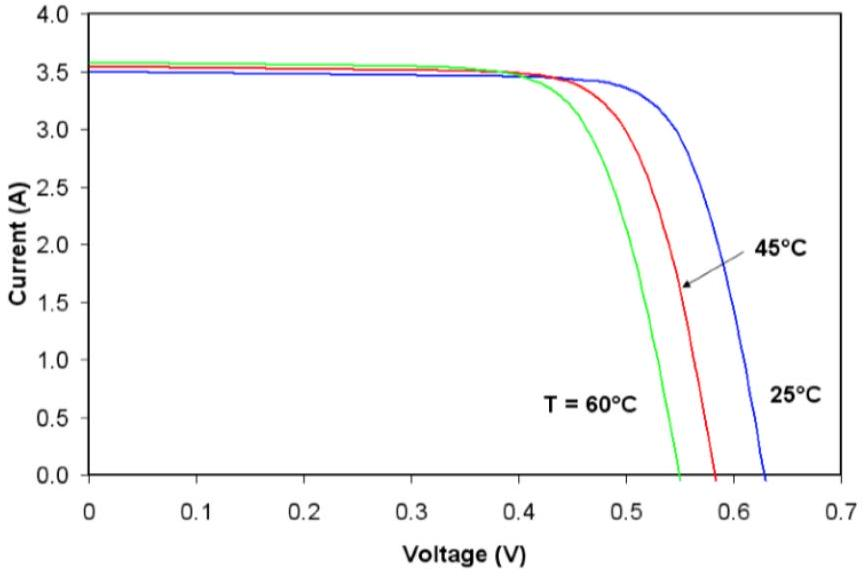
\includegraphics[width=\textwidth]{images/PV_temperature.jpg}\\
    Source: \href{https://en.wikipedia.org/wiki/Theory_of_solar_cells}{Wikipedia}
  \end{column}      
  \begin{column}{0.5\textwidth}
    Effect of irradiance
    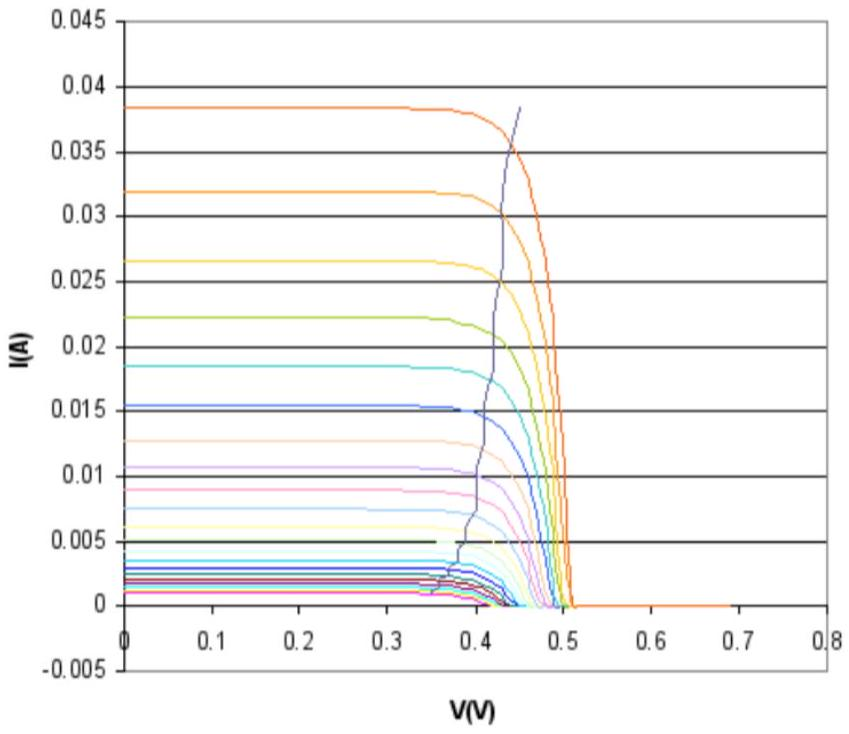
\includegraphics[width=0.8\textwidth]{images/PV_irradiance.jpg}\\
    Source: \href{https://en.wikipedia.org/wiki/Maximum_power_point_tracking}{Wikipedia}
  \end{column}
\end{columns}
\end{frame}

\begin{frame}{Best Research-Cell Efficiencies}
  \begin{center}
    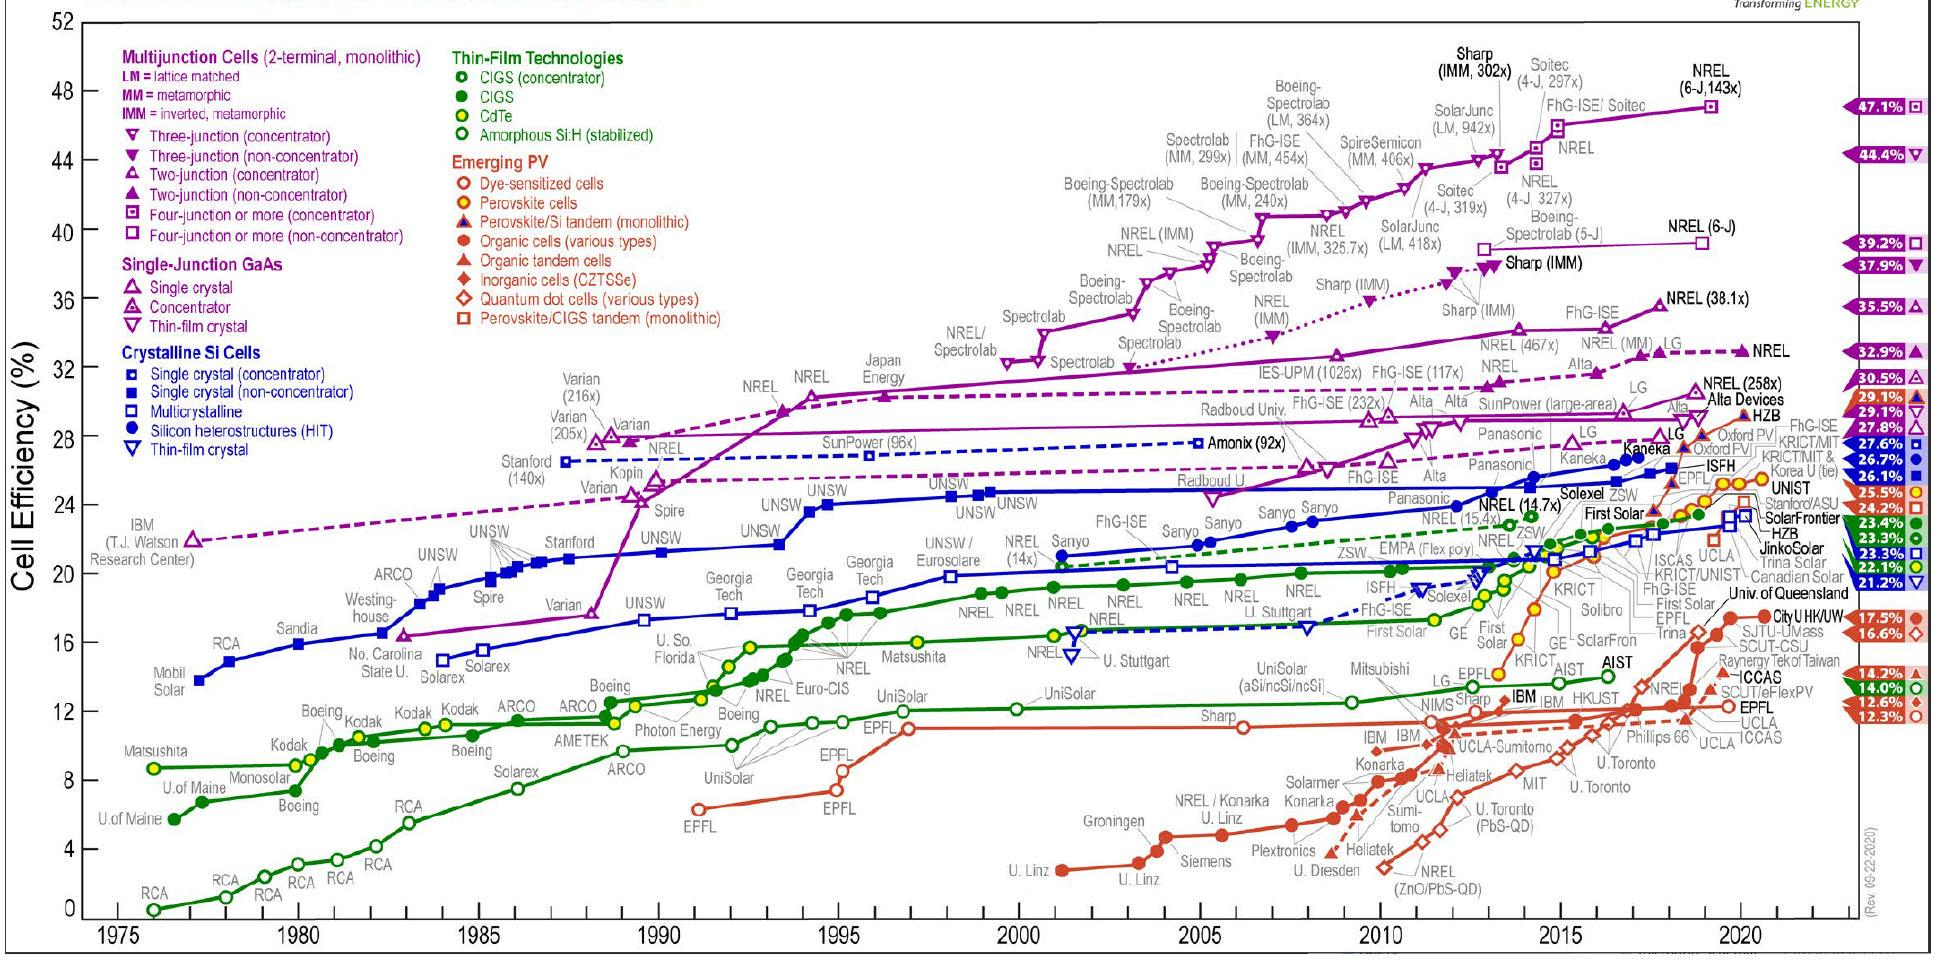
\includegraphics[width=0.8\textwidth]{images/PV_efficiencies.jpg}\\
    Source: \href{https://www.nrel.gov/pv/cell-efficiency.html}{NREL}
  \end{center}
\end{frame}

\begin{frame}{Equivalent electrical model}
\begin{center}
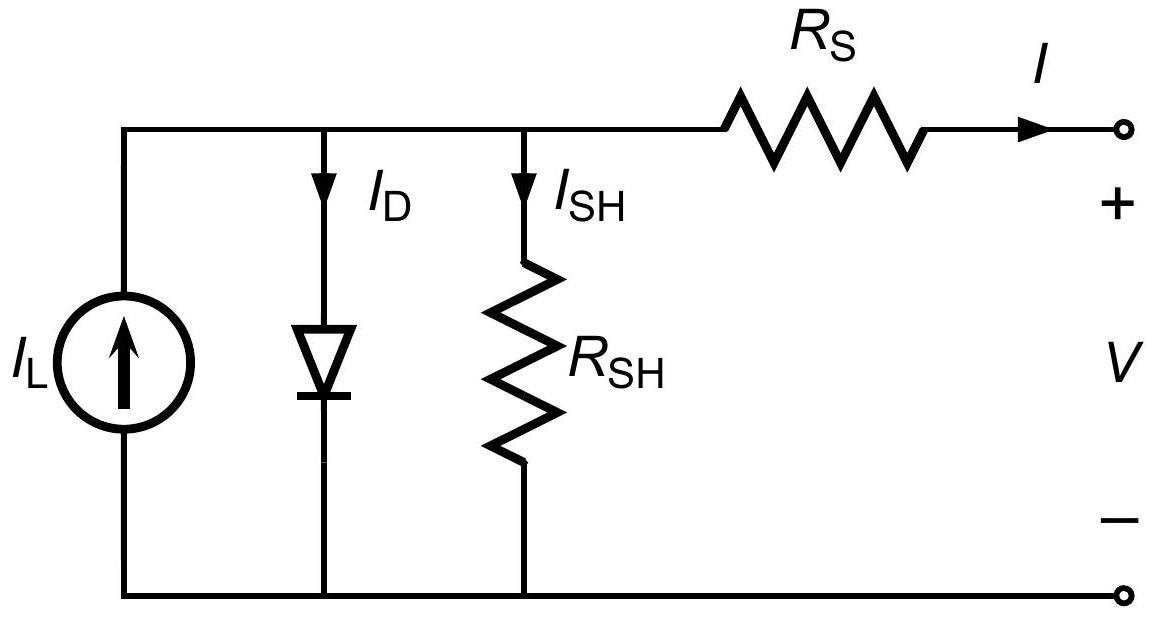
\includegraphics[width=0.4\textwidth]{images/PV_elec_model.jpg}
\end{center}

\begin{itemize}
  \item "It can be shown that for a high-quality solar cell (low $R_{S}$ and $I_{0}$ (diode parameter), and high $R_{S H}$ ) the short-circuit current $I_{S C} \approx I_{L}$ "
  \item The open-circuit voltage is approximately equal to the voltage accross the diode
  \item Both are function of irradiance and temperature
\end{itemize}

Source: \href{https://en.wikipedia.org/wiki/Theory_of_solar_cells}{Wikipedia}

\end{frame}

\begin{frame}  {Maximum power point}
  \centering
  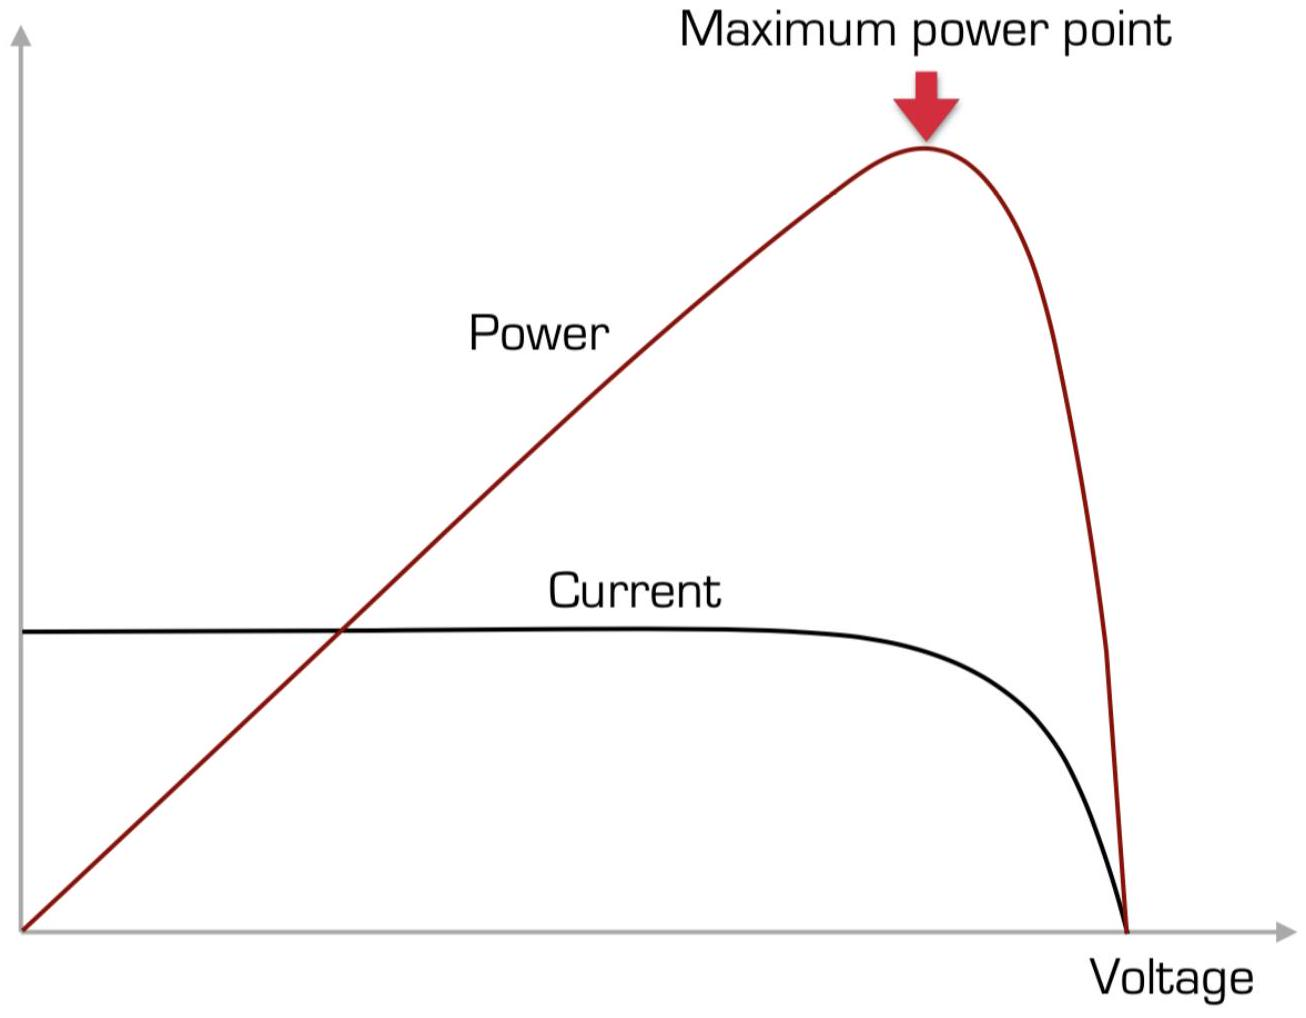
\includegraphics[width=0.6\textwidth]{images/PV_MPPT.jpg}
\end{frame}

\begin{frame}{PV panels}
PV cells are arranged into panels. PV cells are combined in series and in parallel. PV panels are then arranged in parallel and/or in series:

\begin{itemize}
  \item Parallel: same open circuit voltage, increased short circuit current
  \item Series: same short circuit current, increased open circuit voltage, but current limited by PV panel delivering the smallest current.
\end{itemize}

Hence a shadowed or damaged panel can impact the whole array. In practice, PV panels arangement is a mix of series and parallel connections. This trade-off is also impacted by the number and types of power electronics equipment that a particular configuration requires.

\end{frame}

\begin{frame}[allowframebreaks]{Integrating PV arrays}

Extreme approaches:

\begin{columns}
  \begin{column}{0.45\textwidth}
    A single central power electronics interface for entire array:
    \begin{itemize}
      \item low cost in power electronics,
      \item high cost in installation and cabling, low reliability.
      \item Highly impacted by damages, shadow cannot reach MPP per panel
    \end{itemize}
  \end{column}
  \begin{column}{0.45\textwidth}
  One interface for each PV panel (moduleintegrated):
  \begin{itemize}
    \item High cost in power electronics,
    \item low cost in installation and cabling, high reliability.
    \item Robust to damages, shadow
    \item can optimize MPP per panel
  \end{itemize}
  \end{column}
\end{columns}

\newpage
{Realistic approaches:}
\begin{enumerate}
  \item One converter per string
  \item Multiple-input converters
\end{enumerate}
\end{frame}

\begin{frame}{Power electronics interface}
\begin{enumerate}
  \item A DC-DC converter connected at the output of the panel (or string of panels) aiming at reaching the MPP.
  \item An inverter to connect to the grid (or another DC-DC converter if it is a DC bus).
\end{enumerate}
\end{frame}

\begin{frame}[allowframebreaks]{Maximum power point tracking (MPPT)}

  \begin{columns}
  \begin{column}{0.45\textwidth}
    Assume a PV panel feeds a resistor $R_{0}$.\\
    $R_{0}$ is almost never equal to $R_{M P P}=\frac{V_{M P P}}{I_{M P P}}$ since:

    \begin{enumerate}
      \item $R_{0}$ can vary in time depending on the user needs,
      \item $R_{M P P}$ is function of irradiance and temperature.
    \end{enumerate}
  \end{column}
  \begin{column}{0.45\textwidth}
    Hence the panel is usually not naturally operating at its MPP:\\
    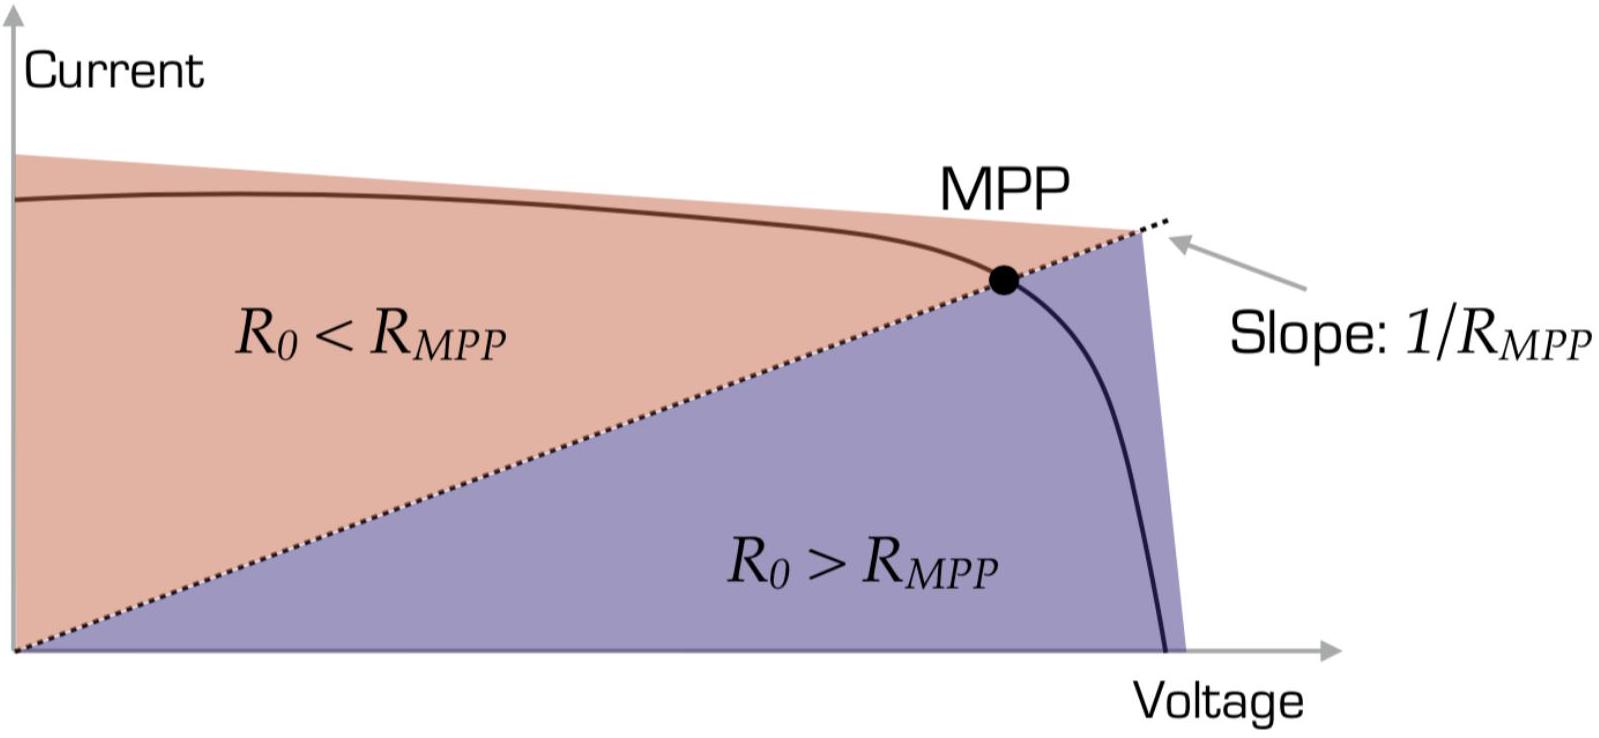
\includegraphics[width=\textwidth]{images/PV_MPP.jpg}
  \end{column}
\end{columns}


To achieve MPP, the DC-DC converter between the PV panel and the resistor is configured to maintain a situation such that the PV panel "sees" a resistance of $R_{M P P}$.

For instance, for a buck converter, it should be $\frac{R_{0}}{D^{2}}$ where $D$ is the duty cycle of the converter. Note that this works only if $R_{M P P}>R_{0}$ since $D \leq 1$.

Several algorithms exist to adapt the value of the duty cycle dynamically.\\
Basic idea: at MPP,

\begin{itemize}
  \item $\frac{d P_{P V}}{d V_{P V}}=0$,
  \item use an iterative algorithm to identify the value of $V_{P V}$ that achieves this.
\end{itemize}

Note that this algorithm works well for a single PV panel, but if a converter is connected to a complex combination of PV panels, several local optima may exist and thus require more advanced solutions.
\end{frame}

\begin{frame}{More on MPPT algorithms}
  \centering
  \href{https://youtu.be/0ItjKs7aJFM}{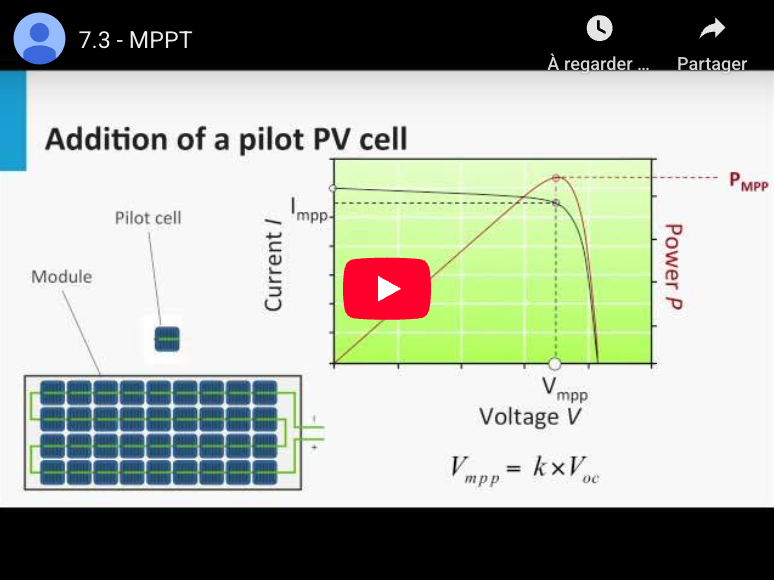
\includegraphics[width=0.6\textwidth]{images/video_MPPT.png}}
\end{frame}



\subsection{Fuel cells}
\begin{frame}{Fuel cells}
A combination (fuel cell + electrolyzer) can be seen as a storage device.\\
We focus here on the electricity (and heat) generation part, i.e. the fuel cell.\\
A fuel cell converts chemical energy directly into electricity. Unlike a battery, it requires a continuous flow of $H_{2}$ fuel:

\begin{itemize}
  \item each $H_{2}$ molecule reacts at the anode and gives two electrons
  \item the remaining $2 H+$ ions pass through the membrane and react with oxygen + electrons coming from the cathode to produce water
\end{itemize}

\end{frame}\begin{frame}{Proton exchange membrane fuel cells (PEMFC)}
These are the most common implementation of fuel cells:

\begin{itemize}
  \item the anode and cathode catalyst is platinum
  \item the membrane is made fof Nafion
\end{itemize}

The reversible voltage is
$$
E_{r}=1.23 \mathrm{~V}
$$

From thermodynamics, it can be shown that the maximum efficiency is
$$
\eta_{\max }=0.83
$$

In practice, its efficiency varies between $35 \%$ and $60 \%$. The main factor affecting its performance is the fuel flow.

\end{frame}\begin{frame}{Fuel cell operation}
\begin{itemize}
  \item Fuels cells have a MPP of operation that corresponds to a cell output voltage of approximately 0.4 V
  \item The power electronics interface must be designed to account for this low cell voltage, hence to provide a high input-output voltage step-up ratio
  \item Another important factor is that the cell must be operated with a relatively constant current output. Else, it can lead to a loss of performance or even to degradation of the membrane and catalysts
\end{itemize}

\subsection{Microturbines}
\end{frame}\begin{frame}{Microturbines}
\begin{itemize}
  \item Moderate cost and efficiency (20\% to $30 \%$ )
  \item Failure rate is relatively low
  \item Moderately fast dynamic response
  \item Usually fueled with natural gas (NG), but can work with other fuels
  \item Units of 20 to 500 kW
\end{itemize}

\end{frame}

\begin{frame}{Working principle of a microturbine}

\begin{columns}
  \begin{column}{0.5\textwidth}
    \begin{enumerate}
      \item Entering air is compressed
      \item It is then mixed with the fuel in a combustion chamber
      \item The mix is ignited, hence the temperature increases and the volume of the air increases
      \item The expanded air actuates the turbine
      \item The turbine drives the shaft of the generator
      \item The heat of the exhausted air is reused to warm the compressed air.
    \end{enumerate}  
  \end{column}
  \begin{column}{0.4\textwidth}
    Microturbines usually follow a \textbf{Brayton} thermodynamic cycle.\\
    Efficiency is affected
    \begin{itemize}
      \item by the temperature ratio between the entering air and the compressed air (hence the reuse of exhaust gases to warm up the air in the compression chamber)
      \item the compression ratio
    \end{itemize}
  \end{column}
\end{columns}

\end{frame}

\begin{frame}{Power electronics interface}
The shaft rotates at a high speed, in the range 50,000 to $120,000 \mathrm{rpm}$. Hence the output voltage of the generator is in the kHz range.

A microtrubines thus requires a rectifier (+ inverter if connected to an AC grid).

\end{frame}


\subsection{Internal combustion engines}
\begin{frame}{Internal combustion engines (ICEs) a.k.a. Gensets}
ICEs are widespread:

\begin{itemize}
  \item low capital cost,
  \item low operation and maintenance costs\footnote{Fuel may nevertheless be very expensive in some parts of the world.}
  \item can be easily moved from one place to another
  \item Can be designed to work with a variety of fuels
  \item Units of several kW to several MW.\\
  \item 

\end{itemize}

\end{frame}\begin{frame}{Working principle of ICEs}
\begin{enumerate}
  \item Intake (induction) stroke
  \item Compression stroke
  \item Power stroke: combustion/expansion
  \item Exhaust stroke
\end{enumerate}

ICEs follow an \textbf{Otto} thermodynamic cycle.
\end{frame}
